\begin{flushright} {\tiny {\color{gray} dgfem1D.tex}} \end{flushright}
%~~~~~~~~~~~~~~~~~~~~~~~~~~~~~~~~~~~~~~~~~~~~~~~~~~~~~~~~~~~~~~~~~~~~~~~~~~~~~~~~~~~~~~~~~~~~~~~~~~


What follows is borrowed from the book "Discontinuous finite elements in fluid dynamics and heat
transfer" by Ben Q. Li \cite{li06}.

To illustrate the basic ideas of the discontinuous finite element method, we
consider a simple, one-dimensional, first order differential equation with $u$
specified at one of the boundaries:
\begin{equation}
\frac{du}{dx} + g =0 \qquad x\in[a,b] \qquad \text{and} \qquad u(x=a)=u_a
\end{equation}
where $g$ is a constant (for simplicity).
The domain is discretized such that : $\Omega_j = [x_j,x_{j+1}]$ with $j = 1, 2, ..., nel$.
Then, integrating the above equation over the element $j$ with respect to a weighting function $f(x)$
\begin{equation}
\int_{x_j}^{x_{j+1}} \left( \frac{d u}{dx} + g \right) f(x) dx = 0
\end{equation}
Remembering that $\int_c^d u(x)v'(x) dx = [u(x)v(x)]_c^d - \int_c^d u'(x)v(x) dx$, 
we can now perform an integration by parts on the differential operator and we obtain:
\begin{equation}
[u(x)f(x)]_{x_j}^{x_{j+1}}  -\int_{x_j}^{x_{j+1}} \left( u \frac{d f}{dx} - g f(x)\right)  dx = 0
\end{equation}
or, 
\begin{equation}
u(x_{j+1})f(x_{j+1}) 
- u(x_{j})f(x_{j}) 
-\int_{x_j}^{x_{j+1}} \left( u \frac{d f}{dx} - g f(x)\right)  dx = 0
\end{equation}


On $\Omega_j$ $u$ is approximated by $u_h \in H$, $H$ being an appropriate function
space of finite dimension, and $f$ by $f_h$ taken from the same function space as $u_h$. 
Upon substituting $(u_h , f_h )$ for $(u,f)$ in the equation above, we have
the discontinuous Galerkin finite element formulation:
\begin{equation}
u_h(x_{j+1}) f_h(x_{j+1}) - u_h(x_{j})f_h(x_{j}) 
-\int_{x_j}^{x_{j+1}} \left( u_h \frac{d f_h}{dx} - g f_h(x)\right)  dx = 0
\end{equation}

In the continuous finite element approach, the field variable $u_h$ is forced to be
continuous across the boundary.
The essential idea for the discontinuous method is
that $u_h$ is allowed to be discontinuous across the boundary. Therefore, across the
element, the following two different values are defined at the two sides of the
boundary:
\begin{equation}
u_j^+ = \lim_{x \searrow x_j^+} u_h(x)
\qquad
u_j^- = \lim_{x \nearrow x_j^-} u_h(x)
\end{equation}

\begin{center}
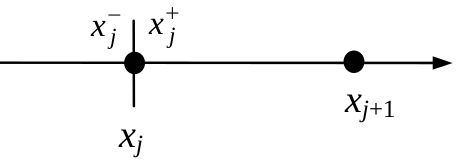
\includegraphics[width=4cm]{images/dgfem/dgfem_1}\\
{\scriptsize An illustration of the jump across $x_j$ of element $j$: 
$x_j$ and $x_{j+1}$ mark the
boundaries of the element}
\end{center}

Conversely, we also have:
\begin{equation}
u_{j+1}^+ = \lim_{x \searrow x_{j+1}^+} u_h(x)
\qquad
u_{j+1}^- = \lim_{x \nearrow x_{j+1}^-} u_h(x)
\end{equation}



It is key to remember that 1) $u_h$ is discontinuous only at the element boundaries; 
2) the solution $u$ is smooth within (but excluding) the boundary. 
By this definition, the above equation contains the variables only within the integral limits of $\Omega_j$ . 
As a consequence, there is no direct coupling with other intervals or other elements. 
{\sl The field values at a node, or the interface between two elements, are not unique}. They are
calculated using the two limiting values approaching the interface from the two
adjacent elements. This feature is certainly desirable for problems with internal
discontinuities.

We can now write CHECK CHECK
\begin{equation}
u_{j+1}^- f_h(x_{j+1}) - u_j^+ f_h(x_{j}) 
-\int_{x_j}^{x_{j+1}} \left( u_h \frac{d f_h}{dx} - g f_h(x)\right)  dx = 0
\end{equation}
and we can integrate by parts again the term which contains a derivative:
\[
\int_{x_j}^{x_{j+1}} u_h(x) \frac{d f_h}{dx} dx = [u_h f_h] -  \int_{x_j}^{x_{j+1}} f_h(x) \frac{d u_h}{dx} dx 
\]

and then 
\begin{equation}
u_{j+1}^- f_h(x_{j+1}) - u_j^+ f_h(x_{j}) 
-\int_{x_j}^{x_{j+1}} \left( u_h \frac{d f_h}{dx} - g f_h(x)\right)  dx = 0
\end{equation}


